\documentclass[12pt,letterpaper]{article}
\usepackage[utf8]{inputenc}
\usepackage[spanish]{babel}
\DeclareUnicodeCharacter{03B5}{\ensuremath{\varepsilon}}
\DeclareUnicodeCharacter{2192}{\ensuremath{\rightarrow}}
\usepackage[top=3.4cm,bottom=3cm,left=3cm,right=3.5cm,headheight=48pt,headsep=14pt]{geometry}
\usepackage{graphicx}
\usepackage{amsmath,amssymb}
\usepackage{booktabs}
\usepackage{float}
\usepackage{caption}
\captionsetup[table]{skip=8pt}
\captionsetup[lstlisting]{skip=4pt}
\usepackage{listings}
\usepackage{fancyhdr}
\usepackage{xcolor}
\usepackage{microtype}
\usepackage[hidelinks]{hyperref}

\graphicspath{{../img/}}

\pagestyle{fancy}
\fancyhf{}
\fancyhead[L]{\small\textit{\nouppercase{\rightmark}}}
\fancyhead[R]{\raisebox{-3pt}{
\includegraphics[height=1.45cm]{escudo_usa.png}}\hspace*{-1.2cm}}
\fancyfoot[C]{\thepage}
\renewcommand{\headrulewidth}{0.5pt}
\fancypagestyle{plain}{\fancyhf{}\fancyfoot[C]{\thepage}\renewcommand{\headrulewidth}{0pt}}

\lstset{
  basicstyle=\ttfamily\small,
  columns=fullflexible,
  keepspaces=true,
  showstringspaces=false,
  breaklines=true,
  xleftmargin=2em,
  aboveskip=0.8em,
  belowskip=0.8em,
  captionpos=t,
  extendedchars=true,
  literate={á}{{\'a}}1 {é}{{\'e}}1 {í}{{\'i}}1 {ó}{{\'o}}1 {ú}{{\'u}}1
           {ñ}{{\~n}}1 {Á}{{\'A}}1 {É}{{\'E}}1 {Í}{{\'I}}1 {Ó}{{\'O}}1
           {Ú}{{\'U}}1 {Ñ}{{\~N}}1 {ü}{{\"u}}1 {¿}{{?`}}1 {¡}{{!`}}1
           {ε}{{$\varepsilon$}}1 {→}{{$\rightarrow$}}1
}

\setlength{\parskip}{0.45em}
\setlength{\parindent}{0pt}
\setlength{\emergencystretch}{3em}

\newcommand{\tk}[1]{\texttt{#1}}
\newcommand{\prim}{\textup{PRIMEROS}}
\newcommand{\sig}{\textup{SIGUIENTES}}
\newcommand{\pred}{\textup{PRED}}

\begin{document}

% ------------------------------------------------------------------ portada
\thispagestyle{plain}
\begin{center}
\vspace*{0.2cm}

\includegraphics[width=0.44\textwidth]{escudo_usa.png}\par
\vspace{2.4cm}
{\LARGE Conjuntos PRIMEROS, SIGUIENTES\\[4pt] y PREDICCIÓN\par}
\vspace{0.5cm}
{\large Análisis sintáctico descendente\par}
\vspace{3.3cm}
{\large\bfseries Lenguajes de programación y traducción\par}
\vspace{0.9cm}
{\bfseries David Andrés Castellanos Angulo\par}
\vspace{2.9cm}
{\itshape Universidad Sergio Arboleda\\
Escuela de ciencias exactas e ingeniería\\
Bogotá D.C., 21 de septiembre de 2026\par}
\end{center}
\newpage

% ------------------------------------------------------------------ 1
\section{Objetivo de la tarea}

El taller pide calcular los conjuntos PRIMEROS y SIGUIENTES de los no terminales de dos gramáticas, y los conjuntos de PREDICCIÓN de sus reglas. Además, el cálculo debe implementarse en Python, leyendo la gramática desde un archivo y no desde la consola.

\begin{figure}[H]
\centering
\begin{minipage}{0.49\textwidth}
  \centering
  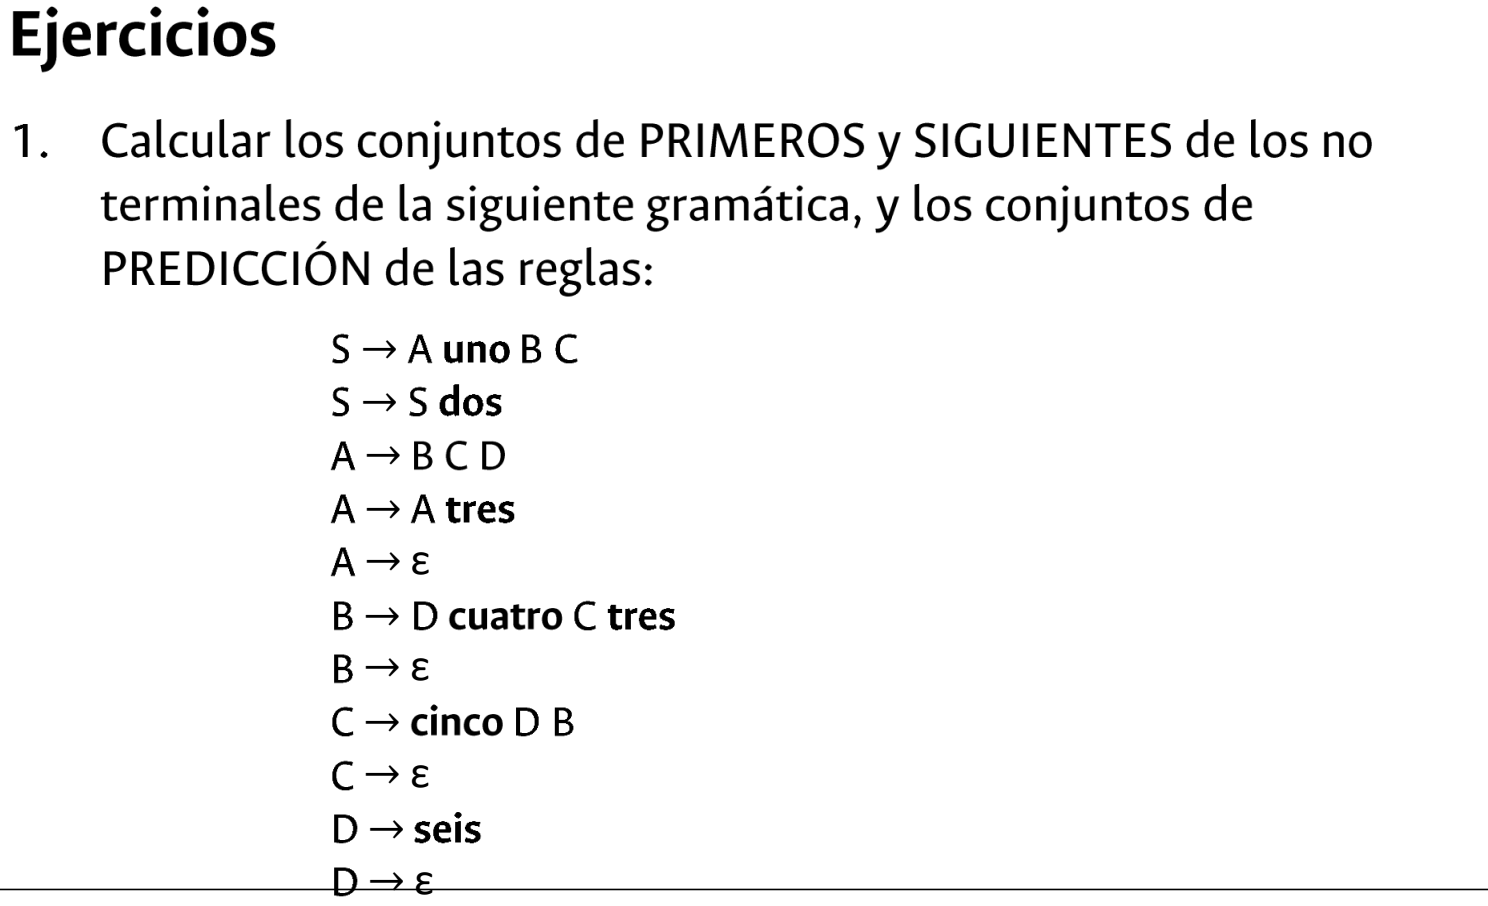
\includegraphics[width=\textwidth]{enunciado_1.png}
\end{minipage}\hfill
\begin{minipage}{0.49\textwidth}
  \centering
  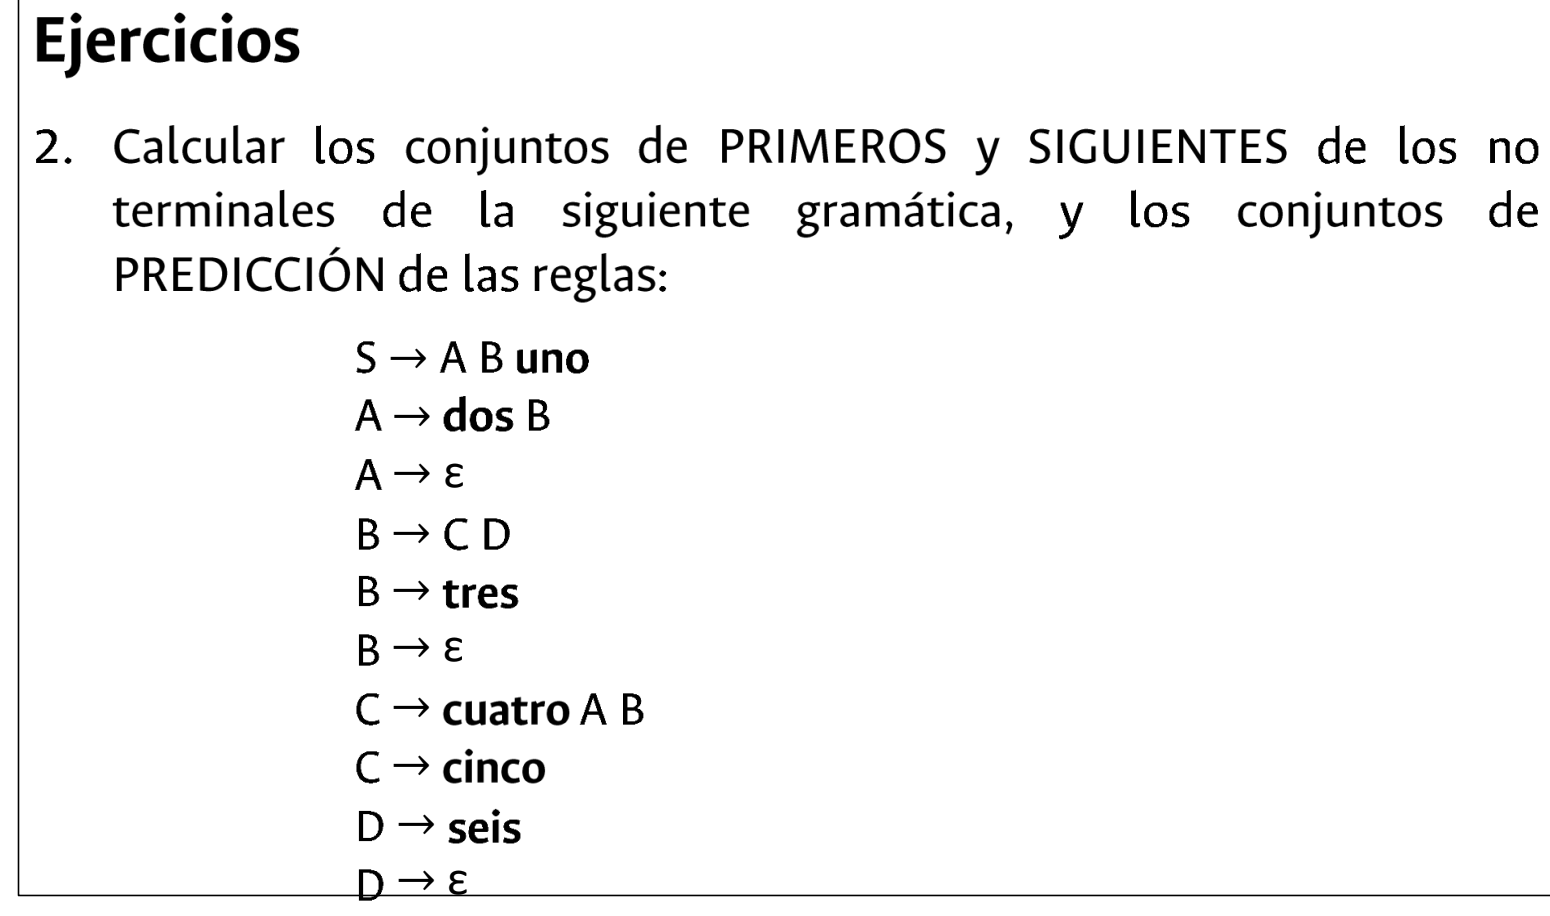
\includegraphics[width=\textwidth]{enunciado_2.png}
\end{minipage}
\caption{Enunciado de los dos ejercicios.}
\end{figure}

Para no depender solo del cálculo a mano, se escribió un programa que sirve para cualquier gramática guardada en un archivo de texto. Con él se resolvieron los dos ejercicios, y sus resultados se contrastaron con el cálculo manual mediante pruebas automáticas.

% ------------------------------------------------------------------ 2
\section{Definiciones}

Siguiendo la notación vista en clase, una gramática se define como $G = (V_N, V_T, S, P)$. Un símbolo es \emph{anulable} si puede derivar la cadena vacía, es decir, si $X \Rightarrow^* \varepsilon$. Sobre esa base se definen los tres conjuntos:

\begin{align*}
\prim(\alpha) &= \{\, a \in V_T \mid \alpha \Rightarrow^* a\beta \,\} \cup \{\, \varepsilon \mid \alpha \Rightarrow^* \varepsilon \,\} \\[2pt]
\sig(A) &= \{\, a \in V_T \cup \{\$\} \mid S \Rightarrow^* \mu A a \nu \,\}
\end{align*}
\begin{alignat*}{2}
\pred(A \rightarrow \alpha) &= \prim(\alpha) &\quad& \text{si $\alpha$ no es anulable}\\[2pt]
\pred(A \rightarrow \alpha) &= \big(\prim(\alpha) - \{\varepsilon\}\big) \cup \sig(A) &\quad& \text{si $\alpha$ es anulable}
\end{alignat*}

PRIMEROS responde con qué terminal puede empezar una cadena, y SIGUIENTES qué terminal puede aparecer justo después de un no terminal; el marcador \tk{\$} representa el fin de la entrada. PREDICCIÓN combina los dos: indica con qué tokens de anticipación es válido elegir cada regla.

% ------------------------------------------------------------------ 3
\section{Entorno e implementación}

Se trabajó en Ubuntu, dentro de una máquina virtual de VirtualBox, con \textbf{Python 3} y sin librerías externas. Todo el cálculo está en \tk{conjuntos.py}.

\subsection{Lectura de la gramática}

El programa recibe la ruta de uno o varios archivos de texto; no pide datos por consola. Cada línea contiene una producción con el formato \tk{A -> X1 X2 ... Xk}. Se aceptan alternativas separadas por \tk{|}, y $\varepsilon$ se puede escribir como \tk{ε} o \tk{eps}. Los no terminales son los símbolos que aparecen a la izquierda de la flecha, el resto son terminales, y el símbolo inicial es el de la primera producción. Si el archivo tiene un error de formato, el programa indica el archivo y la línea.

\subsection{Cálculo de los conjuntos}

Los tres conjuntos se calculan con algoritmos de \textbf{punto fijo}: se recorren todas las reglas agregando elementos, y el recorrido se repite hasta que ningún conjunto cambie. Como los conjuntos solo crecen y la cantidad de símbolos es finita, el proceso siempre termina.

\begin{itemize}
  \item \textbf{PRIMEROS} de una secuencia $X_1 \cdots X_k$: se agrega $\prim(X_i) - \{\varepsilon\}$ de izquierda a derecha hasta llegar al primer símbolo terminal o no anulable. Si todos son anulables, se agrega $\varepsilon$.
  \item \textbf{SIGUIENTES}: se inicia con $\$ \in \sig(S)$. Para cada regla $A \rightarrow \alpha B \beta$ se agrega $\prim(\beta) - \{\varepsilon\}$ a $\sig(B)$; si $\beta$ es vacía o anulable, también se agrega $\sig(A)$.
  \item \textbf{PREDICCIÓN}: se aplica directamente la definición de la sección anterior.
\end{itemize}

La primera regla es la base de las otras dos, porque SIGUIENTES y PREDICCIÓN necesitan los PRIMEROS de secuencias completas.

\noindent\begin{minipage}{\linewidth}
\begin{lstlisting}[language=Python,basicstyle=\ttfamily\footnotesize,caption={PRIMEROS de una secuencia en \texttt{conjuntos.py} (sin anotaciones de tipo).}]
def primeros_de_cadena(simbolos, primeros, no_terminales):
    resultado = set()
    for x in simbolos:
        if x not in no_terminales:      # terminal: aporta solo a sí mismo
            resultado.add(x)
            return resultado
        resultado |= primeros[x] - {EPSILON}
        if EPSILON not in primeros[x]:  # no anulable: aquí termina
            return resultado
    resultado.add(EPSILON)              # todos los símbolos son anulables
    return resultado
\end{lstlisting}
\end{minipage}

\subsection{Ejecución y pruebas}

\noindent\begin{minipage}{\linewidth}
\begin{lstlisting}[caption={Comandos ejecutados en Ubuntu.}]
chmod +x run_all.sh
./run_all.sh                   # pruebas automáticas y los dos ejercicios
python3 conjuntos.py grammars/gramatica1.txt
\end{lstlisting}
\end{minipage}

En \tk{test\_tarea.py} hay 13 pruebas automáticas. Revisan la lectura del archivo (alternativas, $\varepsilon$, comentarios, errores de formato y archivos guardados con BOM), los ejemplos resueltos en clase y los conjuntos completos de los dos ejercicios, calculados a mano. También comprueban dos propiedades que siempre deben cumplirse: $\varepsilon$ nunca pertenece a un conjunto SIGUIENTES, y \tk{\$} siempre pertenece a SIGUIENTES del símbolo inicial. Las 13 pruebas pasan.

% ------------------------------------------------------------------ 4
\section{Ejercicio 1}

La gramática tiene $V_N = \{S, A, B, C, D\}$, $V_T = \{\tk{uno},\allowbreak \tk{dos},\allowbreak \tk{tres},\allowbreak \tk{cuatro},\allowbreak \tk{cinco},\allowbreak \tk{seis}\}$ y símbolo inicial $S$. Así queda escrita en el archivo de entrada:

\noindent\begin{minipage}{\linewidth}
\begin{lstlisting}[caption={\texttt{grammars/gramatica1.txt}.}]
# Ejercicio 1
S -> A uno B C
S -> S dos
A -> B C D
A -> A tres
A -> ε
B -> D cuatro C tres
B -> ε
C -> cinco D B
C -> ε
D -> seis
D -> ε
\end{lstlisting}
\end{minipage}

Son anulables $A$, $B$, $C$ y $D$, porque todos tienen una regla con $\varepsilon$. $S$ no lo es, porque sus dos reglas contienen un terminal.

\begin{table}[H]
\centering
\caption{PRIMEROS y SIGUIENTES del ejercicio 1.}
\small
\begin{tabular}{lll}
\toprule
No terminal & PRIMEROS & SIGUIENTES \\
\midrule
$S$ & \{\texttt{uno}, \texttt{tres}, \texttt{cuatro}, \texttt{cinco}, \texttt{seis}\} & \{\texttt{dos}, \texttt{\$}\} \\
$A$ & \{\texttt{tres}, \texttt{cuatro}, \texttt{cinco}, \texttt{seis}, $\varepsilon$\} & \{\texttt{uno}, \texttt{tres}\} \\
$B$ & \{\texttt{cuatro}, \texttt{seis}, $\varepsilon$\} & \{\texttt{uno}, \texttt{dos}, \texttt{tres}, \texttt{cinco}, \texttt{seis}, \texttt{\$}\} \\
$C$ & \{\texttt{cinco}, $\varepsilon$\} & \{\texttt{uno}, \texttt{dos}, \texttt{tres}, \texttt{seis}, \texttt{\$}\} \\
$D$ & \{\texttt{seis}, $\varepsilon$\} & \{\texttt{uno}, \texttt{dos}, \texttt{tres}, \texttt{cuatro}, \texttt{seis}, \texttt{\$}\} \\
\bottomrule
\end{tabular}
\end{table}

Para PRIMEROS conviene empezar por los no terminales cuyas reglas arrancan con un terminal: $D$ y $C$ aportan \tk{seis} y \tk{cinco}. En $B \rightarrow D\ \tk{cuatro}\ C\ \tk{tres}$, $D$ es anulable, así que además de \tk{seis} entra \tk{cuatro}. En $A \rightarrow B\,C\,D$ los tres símbolos son anulables, por lo que $A$ recoge \tk{cuatro}, \tk{seis} y \tk{cinco}, y además $\varepsilon$. El caso menos obvio es $A \rightarrow A\ \tk{tres}$: como $A$ es anulable, \tk{tres} también puede quedar al inicio y entra en $\prim(A)$. Por último, $S$ recibe $\prim(A)$ sin $\varepsilon$ y, como $A$ es anulable, también \tk{uno}.

En SIGUIENTES, el que recibe de más lugares es $B$. En $S \rightarrow A\ \tk{uno}\ B\,C$ le sigue $C$, que aporta \tk{cinco} y, por ser anulable, deja pasar $\sig(S)$. En $A \rightarrow B\,C\,D$ le siguen $C$ y $D$, que aportan \tk{cinco} y \tk{seis} y dejan pasar $\sig(A)$. Y en $C \rightarrow \tk{cinco}\ D\,B$ queda al final, así que recibe $\sig(C)$.

\begin{table}[H]
\centering
\caption{Conjuntos de PREDICCIÓN del ejercicio 1.}
\small
\begin{tabular}{rll}
\toprule
\# & Regla & PREDICCIÓN \\
\midrule
1 & $S \rightarrow$ $A$\ \texttt{uno}\ $B$\ $C$ & \{\texttt{uno}, \texttt{tres}, \texttt{cuatro}, \texttt{cinco}, \texttt{seis}\} \\
2 & $S \rightarrow$ $S$\ \texttt{dos} & \{\texttt{uno}, \texttt{tres}, \texttt{cuatro}, \texttt{cinco}, \texttt{seis}\} \\
3 & $A \rightarrow$ $B$\ $C$\ $D$ & \{\texttt{uno}, \texttt{tres}, \texttt{cuatro}, \texttt{cinco}, \texttt{seis}\} \\
4 & $A \rightarrow$ $A$\ \texttt{tres} & \{\texttt{tres}, \texttt{cuatro}, \texttt{cinco}, \texttt{seis}\} \\
5 & $A \rightarrow$ $\varepsilon$ & \{\texttt{uno}, \texttt{tres}\} \\
6 & $B \rightarrow$ $D$\ \texttt{cuatro}\ $C$\ \texttt{tres} & \{\texttt{cuatro}, \texttt{seis}\} \\
7 & $B \rightarrow$ $\varepsilon$ & \{\texttt{uno}, \texttt{dos}, \texttt{tres}, \texttt{cinco}, \texttt{seis}, \texttt{\$}\} \\
8 & $C \rightarrow$ \texttt{cinco}\ $D$\ $B$ & \{\texttt{cinco}\} \\
9 & $C \rightarrow$ $\varepsilon$ & \{\texttt{uno}, \texttt{dos}, \texttt{tres}, \texttt{seis}, \texttt{\$}\} \\
10 & $D \rightarrow$ \texttt{seis} & \{\texttt{seis}\} \\
11 & $D \rightarrow$ $\varepsilon$ & \{\texttt{uno}, \texttt{dos}, \texttt{tres}, \texttt{cuatro}, \texttt{seis}, \texttt{\$}\} \\
\bottomrule
\end{tabular}
\end{table}

\begin{figure}[H]
\centering
\begin{minipage}{0.48\textwidth}
  \centering
  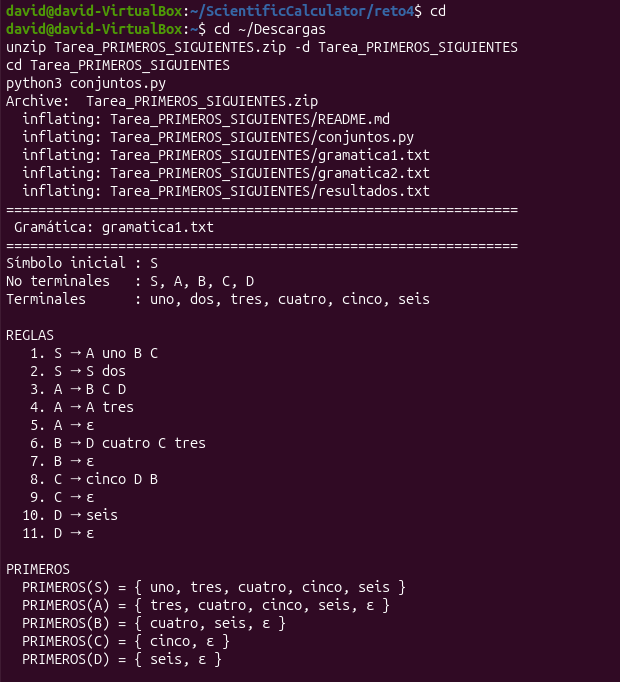
\includegraphics[width=\textwidth]{evid_ejecucion.png}
\end{minipage}\hfill
\begin{minipage}{0.48\textwidth}
  \centering
  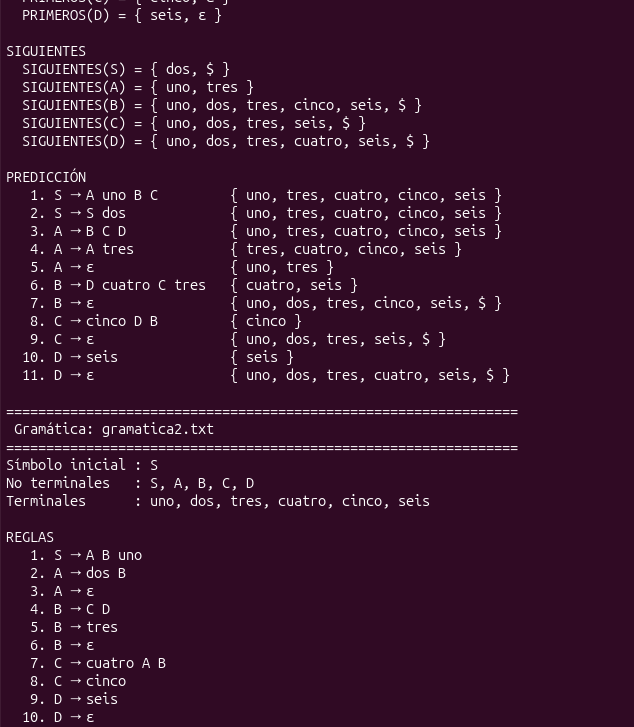
\includegraphics[width=\textwidth]{evid_ejercicio1.png}
\end{minipage}
\caption{Ejecución del ejercicio 1 en Ubuntu. A la izquierda, la lectura de la gramática y PRIMEROS; a la derecha, SIGUIENTES y PREDICCIÓN.}
\end{figure}

% ------------------------------------------------------------------ 5
\section{Ejercicio 2}

Los terminales y no terminales son los mismos del ejercicio 1, y el símbolo inicial sigue siendo $S$.

\noindent\begin{minipage}{\linewidth}
\begin{lstlisting}[caption={\texttt{grammars/gramatica2.txt}.}]
# Ejercicio 2
S -> A B uno
A -> dos B
A -> ε
B -> C D
B -> tres
B -> ε
C -> cuatro A B
C -> cinco
D -> seis
D -> ε
\end{lstlisting}
\end{minipage}

Son anulables $A$, $B$ y $D$. $C$ no lo es, porque sus dos reglas empiezan con un terminal, y $S$ tampoco, porque su única regla termina en \tk{uno}.

\begin{table}[H]
\centering
\caption{PRIMEROS y SIGUIENTES del ejercicio 2.}
\small
\begin{tabular}{lll}
\toprule
No terminal & PRIMEROS & SIGUIENTES \\
\midrule
$S$ & \{\texttt{dos}, \texttt{tres}, \texttt{cuatro}, \texttt{cinco}, \texttt{seis}\} & \{\texttt{\$}\} \\
$A$ & \{\texttt{dos}, $\varepsilon$\} & \{\texttt{uno}, \texttt{tres}, \texttt{cuatro}, \texttt{cinco}, \texttt{seis}\} \\
$B$ & \{\texttt{tres}, \texttt{cuatro}, \texttt{cinco}, \texttt{seis}, $\varepsilon$\} & \{\texttt{uno}, \texttt{tres}, \texttt{cuatro}, \texttt{cinco}, \texttt{seis}\} \\
$C$ & \{\texttt{cuatro}, \texttt{cinco}\} & \{\texttt{uno}, \texttt{tres}, \texttt{cuatro}, \texttt{cinco}, \texttt{seis}\} \\
$D$ & \{\texttt{seis}, $\varepsilon$\} & \{\texttt{uno}, \texttt{tres}, \texttt{cuatro}, \texttt{cinco}, \texttt{seis}\} \\
\bottomrule
\end{tabular}
\end{table}

Para PRIMEROS se siguió el desarrollo hecho en clase, agrupando por reglas: $\prim(B) = \{\tk{tres}, \varepsilon\} \cup \big(\prim(CD) - \{\varepsilon\}\big)$ y $\prim(S) = \prim(AB) - \{\varepsilon\}$. De ahí salen los conjuntos de la tabla anterior.

En SIGUIENTES aparece una dependencia cíclica. Por $C \rightarrow \tk{cuatro}\ A\,B$, con $B$ anulable, $\sig(C)$ pasa a $A$ y a $B$; por $B \rightarrow C\,D$, con $D$ anulable, $\sig(B)$ pasa a $C$ y a $D$; y por $A \rightarrow \tk{dos}\ B$, $\sig(A)$ pasa a $B$. Como $A$, $B$ y $C$ se alimentan entre sí, el punto fijo los deja iguales, y $D$ termina igual a $B$. Ninguno contiene \tk{\$}: $S$ no aparece en el lado derecho de ninguna regla y toda cadena del lenguaje termina en \tk{uno}.

\begin{table}[H]
\centering
\caption{Conjuntos de PREDICCIÓN del ejercicio 2.}
\small
\begin{tabular}{rll}
\toprule
\# & Regla & PREDICCIÓN \\
\midrule
1 & $S \rightarrow$ $A$\ $B$\ \texttt{uno} & \{\texttt{uno}, \texttt{dos}, \texttt{tres}, \texttt{cuatro}, \texttt{cinco}\} \\
2 & $A \rightarrow$ \texttt{dos}\ $B$ & \{\texttt{dos}\} \\
3 & $A \rightarrow$ $\varepsilon$ & \{\texttt{uno}, \texttt{tres}, \texttt{cuatro}, \texttt{cinco}, \texttt{seis}\} \\
4 & $B \rightarrow$ $C$\ $D$ & \{\texttt{cuatro}, \texttt{cinco}\} \\
5 & $B \rightarrow$ \texttt{tres} & \{\texttt{tres}\} \\
6 & $B \rightarrow$ $\varepsilon$ & \{\texttt{uno}, \texttt{tres}, \texttt{cuatro}, \texttt{cinco}, \texttt{seis}\} \\
7 & $C \rightarrow$ \texttt{cuatro}\ $A$\ $B$ & \{\texttt{cuatro}\} \\
8 & $C \rightarrow$ \texttt{cinco} & \{\texttt{cinco}\} \\
9 & $D \rightarrow$ \texttt{seis} & \{\texttt{seis}\} \\
10 & $D \rightarrow$ $\varepsilon$ & \{\texttt{uno}, \texttt{tres}, \texttt{cuatro}, \texttt{cinco}, \texttt{seis}\} \\
\bottomrule
\end{tabular}
\end{table}

\begin{figure}[H]
\centering
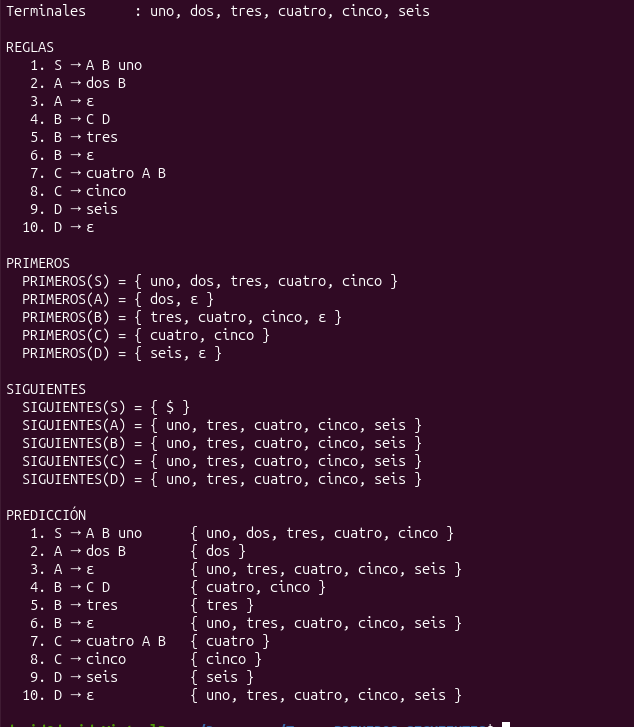
\includegraphics[width=0.56\textwidth]{evid_ejercicio2.png}
\caption{Ejecución del ejercicio 2 en Ubuntu.}
\end{figure}

% ------------------------------------------------------------------ 6
\section{Análisis}

De los dos ejercicios se pueden sacar tres observaciones.

La primera es que la anulabilidad es lo que más influye en el cálculo. En el ejercicio 1, cuatro de los cinco no terminales son anulables, y por eso casi todos los conjuntos terminan grandes: PRIMEROS de una regla depende de varios símbolos seguidos, y SIGUIENTES se propaga de un no terminal a otro. En el ejercicio 2 el cálculo se agrupó por reglas, tomando los PRIMEROS de cada lado derecho completo.

La segunda es que el algoritmo de punto fijo evita tener que ordenar el cálculo. En el ejercicio 2 no hay un orden que permita calcular SIGUIENTES de una sola pasada, porque $A$, $B$ y $C$ dependen unos de otros. Con el punto fijo se repiten las pasadas hasta que ningún conjunto crece, sin decidir nada a mano.

La tercera es que \tk{\$} marca dónde puede terminar la entrada. En el ejercicio 1 aparece en SIGUIENTES de $B$, $C$ y $D$, porque cualquiera de ellos puede quedar al final de una forma sentencial. En el ejercicio 2 solo está en $\sig(S)$, porque después de cualquier otro no terminal siempre falta por lo menos el \tk{uno} final.

% ------------------------------------------------------------------ 7
\section{Conclusiones}

\begin{itemize}
  \item Se implementó en Python un programa que lee una gramática desde un archivo y calcula sus terminales, no terminales, PRIMEROS, SIGUIENTES y PREDICCIÓN. Con él se resolvieron los dos ejercicios.
  \item Todos los conjuntos se calculan con punto fijo, lo que resuelve dependencias cíclicas como las del ejercicio 2 sin ordenar el cálculo a mano.
  \item La anulabilidad determina hasta dónde se propagan los conjuntos: un solo símbolo no anulable, como $C$ en el ejercicio 2, basta para cortar PRIMEROS de una regla.
  \item Las 13 pruebas automáticas confirman los resultados del cálculo manual y verifican propiedades que siempre deben cumplirse, como que $\varepsilon$ nunca aparece en SIGUIENTES.
\end{itemize}

\end{document}
